\documentclass[]{scrreprt}
\usepackage{amsmath,amsfonts,graphicx}
\usepackage{multirow}
\usepackage{pslatex}
\usepackage{tabularx}
\usepackage{comment}
\usepackage{xspace}
\usepackage{array}

\usepackage{hyperref}

\usepackage{caption}
\DeclareCaptionFont{white}{\color{white}}
\DeclareCaptionFormat{listing}{\colorbox{gray}{\parbox{\textwidth}{#1#2#3}}}

\graphicspath{
{figures/}
}

\newcommand{\uo}{\mbox{UO\textsubscript{2}}\xspace}

\setcounter{secnumdepth}{3}

\newcommand{\si}{\sigma}
\newcommand{\mand}{\ \ \ \mbox{and}\ \ \ }
\newcommand{\pl}{\partial}
\newcommand{\ha}{\mbox{$\frac{1}{2}$}}
\newcommand{\thetac}{\theta^{\mathrm{c}}}
\newcommand{\thetarel}{\theta^{\mathrm{rel}}}
\newcommand{\ep}{\epsilon}
\newcommand{\ga}{\gamma}
\newcommand{\spa}{\ \ \ }
\newcommand{\non}{\nonumber}
\newcommand{\de}{\delta}
\newcommand{\ka}{\kappa}
\newcommand{\la}{\lambda}
\newcommand{\tr}{\mbox{Tr}\,}
\newcommand{\al}{\alpha}
\newcommand{\be}{\beta}
\newcommand{\cd}{\cdot}

\begin{document}


\title{Cosserat Test suite}
\author{CSIRO}
\maketitle

\abstract{Tests involving Cosserat mechanics are described.  The
  notation is defined in the Theory manual.}

\tableofcontents

\chapter{Cosserat glide: elasticity}

Forest\footnote{S Forest "Mechanics of Cosserat media An
  introduction".  Available from
  http://citeseerx.ist.psu.edu/viewdoc/download?doi=10.1.1.154.4476\&rep=rep1\&type=pdf}
describes a ``glide'' test of Cosserat elasticity in his Appendix A.
The test involves a 3D material, but all quantities are assumed to be
functions of the $x_{2} = y$ direction only.
The displacement field, $u$, and Cosserat rotation, $\thetac$
are assumed to obey
\begin{eqnarray}
u_{i} & = & (u_{x}(y),\ 0,\ 0) \ , \\
\thetac_{i} & = & (0,\ 0,\ \thetac_{z}(y)) \ .
\end{eqnarray}
These mean that the strain tensor, $\gamma$, and curvature tensor, $\kappa$, are
\begin{eqnarray}
\gamma = \left(
\begin{array}{ccc}
0 & \thetac_{z} + \nabla_{y}u_{x} & 0 \\
-\thetac_{z} & 0 & 0 \\
0 & 0 & 0
\end{array}
\right)
&&
\kappa = \left(
\begin{array}{ccc}
0 & 0 & 0 \\
0 & 0 & 0 \\
0 & \nabla_{y}\thetac_{z} & 0
\end{array}
\right)
\end{eqnarray}
The solution below has boundary conditions $u_{x}(0) = 0 =
\thetac_{z}(y)$.

The stress and couple-stress tensors are assumed to be zero, except for
the following components:
\begin{eqnarray}
\sigma_{yx} & \neq & 0 \ , \\
m_{zy} & \neq & 0 \ .
\end{eqnarray}
If standard (non-Cosserat, Cauchy) elasticity were being
used, the solution is the trivial $u_{x} = 0$.  However, using
Cosserat elasticity a nontrivial solution is found.
Physically this setup corresponds to a 3D object with infinite extent
in the $x$ and $z$ directions subjected to a moment $m_{zy}$ that
rotates the Cosserat grains.  The 3D object may or may not be finite
in the $y$ direction.  The MOOSE simulation actually uses a unit
cube of material: the infiniteness in the $x$ and $z$ directions
is irrelevant since there is no dependence of the variables on these
directions.

Isotropic elasticity is assumed, with the additional assumption that
the couple-stress equation only involves two moduli:
\begin{eqnarray}
\si_{ij} & = & \la\de_{ij}\tr\ga + 2\mu\ga_{(ij)} + 2\al\ga_{[ij]} \ ,
\non \\
m_{ij} & = & \be\de_{ij}\tr\ka + 2\ep\ka_{(ij)} + 2\ep\ka_{[ij]} \ .
\end{eqnarray}
With these assumptions, the moment and force balance equations reduce
to a second-order ODE that has solution
\begin{eqnarray}
\thetac_{z} & = & B\sinh(\omega_{e}y) \ , \\
u_{x} & = & \frac{2 \al B}{\omega_{e}(\mu + \al)}(1 -
\cosh(\omega_{e}y)) \ , \\
m_{zy} & = & 2B\epsilon \omega_{e}\cosh(\omega_{e}y) \ , \\
\sigma_{yx} & = & -\frac{4\mu\al}{\mu + \al}B\sinh(\omega_{e}y)
\end{eqnarray}
with $B$ being an arbitrary constant of integration, and
\begin{equation}
\omega_{e} = \sqrt{\frac{2\mu\al}{\epsilon(\mu + \al)}} \ .
\end{equation}
Forest's notation is slightly different: for $\al$ he writes $\mu_{c}$,
and for $\epsilon$ he writes $\beta$.

The MOOSE simulation uses 100 elements in the $y$ direction, with
$\mu=2$, $\al=3$ and $\epsilon=0.6$.  This gives $w_{e}=2$.  Preset
boundary conditions at $y=0$ and $y=1$ are used, and the system
relaxes to the equilirium solution within 1 iteration.
Figure~\ref{glide_elast.fig} reveals that the MOOSE simulation agrees
with expectations.  The displacements agree well for the 100-element
simulation, but the stress components agree less well (this is not
really observable to the eye in Figure~\ref{glide_elast.fig}) and even a
non-zero $\sigma_{xy}$ appears.  However, as the number of elements
is increased, the stresses tend to the analytical formulae given above.

\begin{figure}[htb]
\begin{center}
\begin{tabular}{cc}
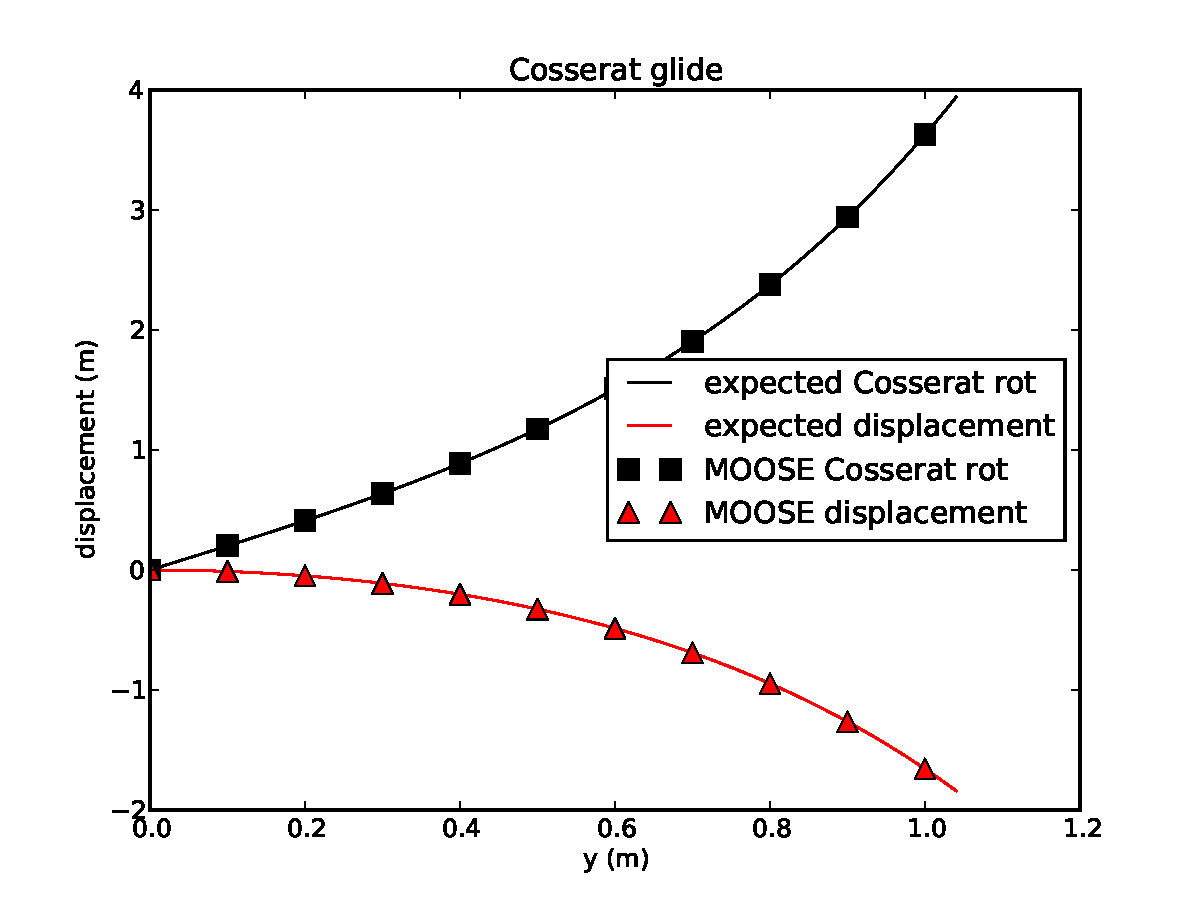
\includegraphics[width=8cm]{cosserat_glide_disp.pdf}
&
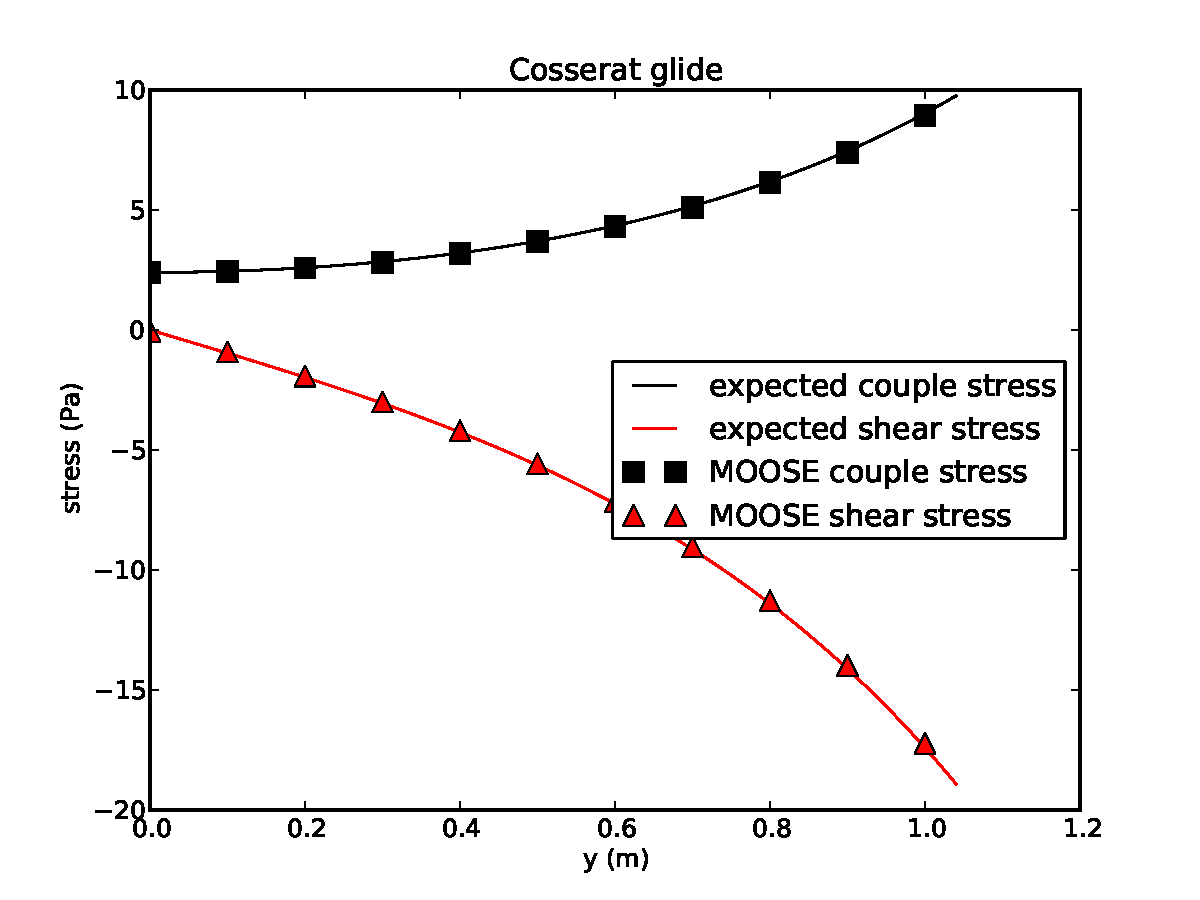
\includegraphics[width=8cm]{cosserat_glide_stress.pdf}
\end{tabular}
\caption{Results from the elastic Cosserat glide test.  Left:
  displacements.  Right: stresses}
\label{glide_elast.fig}
\end{center}
\end{figure}


\chapter{Cosserat tension}

This is a simple test where a 3D sample is subjected to a normal load
on its top surface.  The sample is allowed to shrink in directions
perpendicular to the force, via the Poisson's ratio.  Specifically,
all components of the stress tensor are zero except for
\begin{equation}
\sigma_{22} \neq 0 \ ,
\end{equation}
(which is constant).
There are no Cosserat rotations involved:
\begin{equation}
m = 0 = \kappa \ .
\end{equation}
A general isotropic elasticity tensor is assumed so that the
constitutive relation reads
\begin{equation}
\si_{ij} = \la\de_{ij}\tr\ga + 2\mu\ga_{(ij)} + 2\al\ga_{[ij]} \ .
\end{equation}
The solution is identical to the standard (non-Cosserat) case, which
is independent of $\al$, and has strain components
\begin{equation}
\epsilon_{22} = \frac{(\la + \mu)}{\mu(3\la + 2\mu)}\sigma_{22}
\ \ \ \mbox{and}\ \ \
\epsilon_{11} = \epsilon_{33} = -\frac{\la}{2(\mu + \la)}\epsilon_{22}
\ .
\end{equation}
MOOSE generates this solution exactly.




\end{document}

